\chapter{Literature Review}\label{ch:lit}\addtocontents{lof}{\protect\contentsline{chapter}{\protect\numberline{\thechapter}Literature Review}{}{}}\addtocontents{lot}{\protect\contentsline{chapter}{\protect\numberline{\thechapter}Literature Review}{}{}}


% \openepigraph{Sound, a certain movement of air.}{Aristotele, De Anima II.8 420b12}
\vspace{-2.5em}
% \newthought{Synopsis}\synopsisChAcoustics

\mynewline

% Heart Valve Anatomy and Physiology
\section{Heart Valve Anatomy and Physiology}

\subsection{Introduction to the Heart Valve System}
%     Introduction to the Heart Valve System: Start by providing a general overview of the heart's valve system, including its role in the circulatory system. Highlight the importance of valve function for cardiovascular health.
The heart valve system plays a pivotal role in the circulatory system, ensuring the unidirectional flow of blood through the heart and maintaining cardiovascular health. The cardiovascular system, as a closed circulatory network, is divided into two primary circuits: one that pumps blood from the heart to the lungs for oxygenation, the right, and another that distributes this oxygenated blood to the body's organs, the left. The heart is composed of four chambers: two atria for receiving blood and two ventricles for pumping blood to the body. To maintain the blood's unidirectional flow, the heart has a valve in each chamber each of which are unique to the geometry of the chamber and have their own unique pathologies, they're strategically located between the atria and ventricles and between the ventricles and the arteries that emerge from the heart. ~\citeonly{fraterARTIFICIALHEARTVALVES1962}
\marginpar{
    \centering
    \footnotesize
    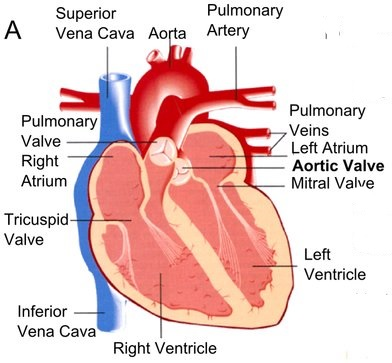
\includegraphics[width=\linewidth]{figures/heartimage.jpg}
    \captionof{figure}{Heart Valve System ~\citeonly{rockComplexCollagenFiber2014}}
    \label{fig:heart_valves}
}

The functionality and integrity of heart valves are essential for cardiovascular health. Heart valves open and close with each heartbeat, totaling over 3 billion times in a lifetime. This continuous operation occurs under significant pressure and within flowing blood, a viscous fluid rich in minerals, proteins, lipids, and cells. When valves become defective, they critically affect heart performance, leading to valve diseases that necessitate surgical intervention in the absence of curative drug treatments. Currently, diseased valves are replaced with artificial devices designed to emulate the valves' mechanical functions and restore heart functionality. However, these artificial valves can fail due to design flaws, material imperfections, or biocompatibility issues, often requiring risky reoperations. ~\citeonly{simionescuArtificialHeartValves2006}

Biomedical engineering strives to enhance treatments for valvular diseases, potentially impacting millions worldwide. This interdisciplinary field combines efforts from medicine, biology, engineering, and mechanics to improve device biocompatibility and explore tissue-engineering approaches that could enable the complete regeneration of valve tissues. ~\citeonly{simionescuArtificialHeartValves2006}

% \mynewline
% In summary, the heart valve system is central to the efficient operation of the cardiovascular system, ensuring that blood flows correctly throughout the body. The ongoing challenge in biomedical engineering is to develop better treatments for valvular diseases, aiming to improve or replace the natural function of heart valves effectively.

\subsection{Anatomy of the tricuspid valve}
%     Detailed Anatomy of the \gls{TV}: Focus on the \gls{TV}, given your project's emphasis. Describe its location, structure (leaflets, annulus, chordae tendineae, papillary muscles), and how these components work together to ensure unidirectional blood flow.
The \gls{TV}, an integral component of the heart's valve system, is located between the right atrium and right ventricle. It plays a crucial role in ensuring unidirectional blood flow from the atrium to the ventricle, thus maintaining the efficiency of the cardiac cycle. The \gls{TV}'s anatomy is complex and consists of several key structures: the annulus, leaflets, chordae tendineae, and papillary muscles.
\marginpar{
    \centering
    \footnotesize
    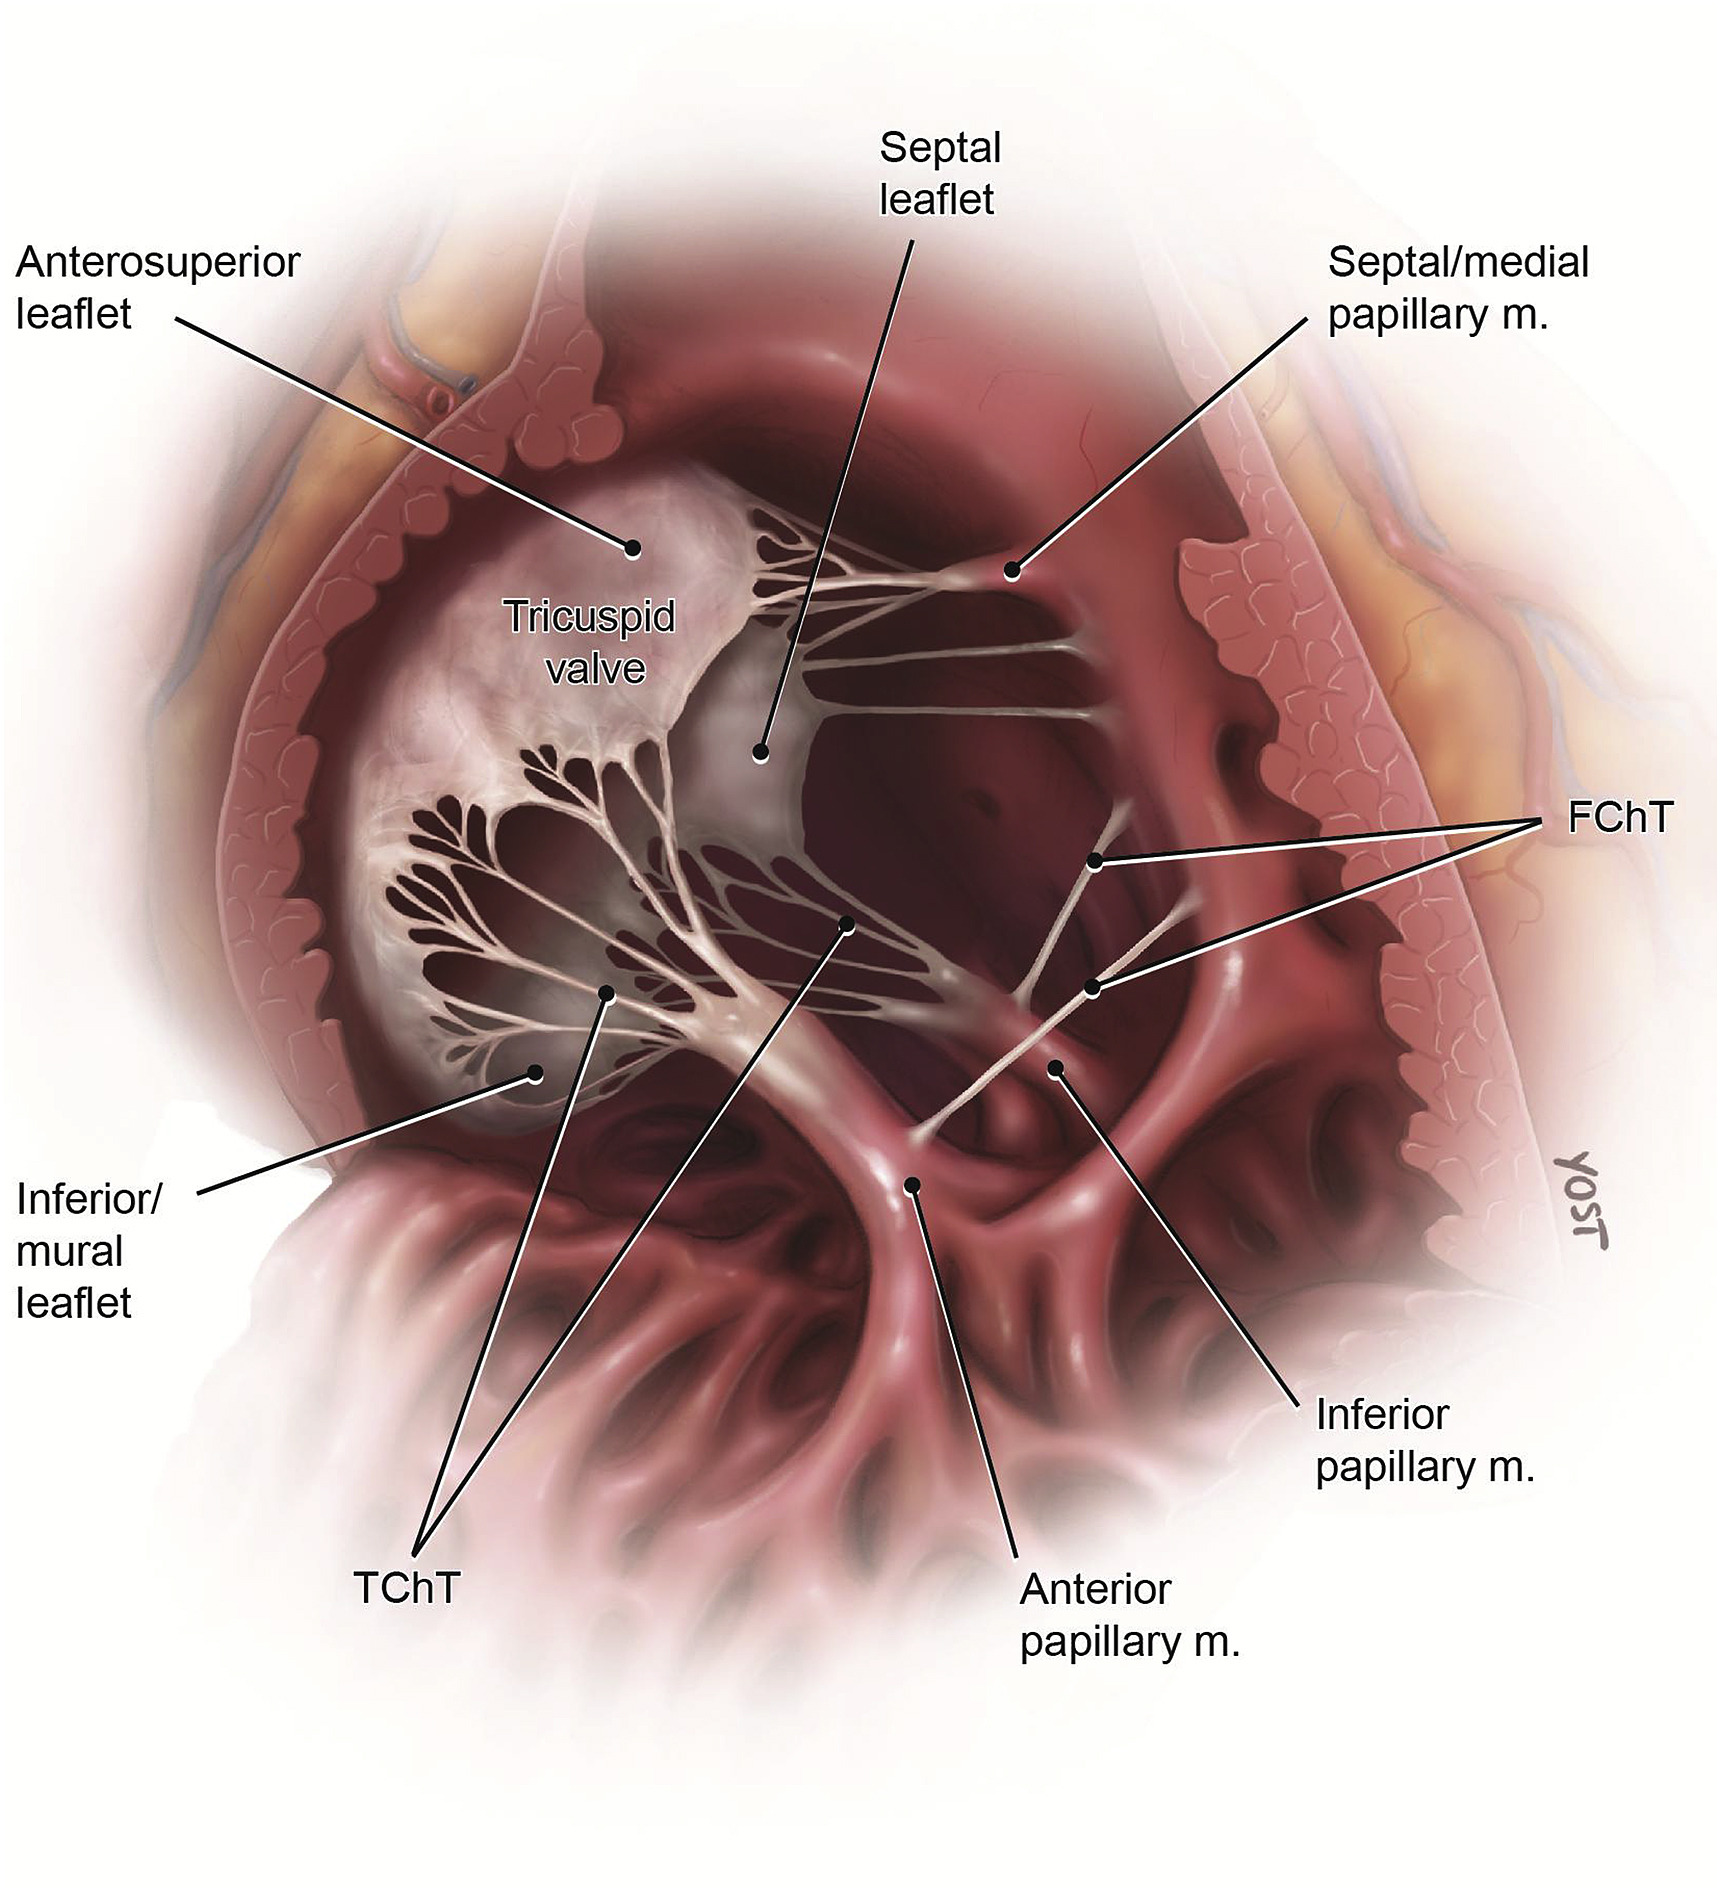
\includegraphics[width=\linewidth]{figures/tricuspidimage.jpg}
    \captionof{figure}{Sub-System of Tricuspid Valve ~\citeonly{YostDrawingDetailed}}
    \label{fig:tricuspid_valve}
}

\begin{itemize}
    \item Annulus: The annulus is a fibrous ring that anchors the valve leaflets and maintains their spatial configuration. It is the foundation to which the leaflets are attached, providing structural support for the entire valve apparatus.

    \item Leaflets: Typically, the \gls{TV} has three leaflets named according to their position: the anterior, posterior, and septal leaflets. These leaflets act as one-way doors that open to allow blood flow from the atrium to the ventricle and close to prevent backflow.

    \item Chordae Tendineae: These are thin, string-like structures that connect the valve leaflets to the papillary muscles. The chordae tendineae ensure the leaflets close securely and prevent them from inverting when the ventricle contracts.

    \item Papillary Muscles: These muscles extend from the inner walls of the right ventricle and attach to the valve leaflets via the chordae tendineae. During ventricular contraction, the papillary muscles contract, pulling the chordae tendineae taut and ensuring the valve leaflets close properly.
\end{itemize}

The \gls{TV}'s structure is characterized by its adaptability and variability. The number, length, and shape of the chordae tendineae and the papillary muscles can vary significantly among individuals, which can be of clinical significance. Dysfunctional papillary muscles or dysplastic chordae can lead to valve dysfunction, emphasizing the importance of understanding this complex anatomy for clinical assessment and intervention ~\citeonly{sandersTricuspidValveEmbryology2014}

Furthermore, the \gls{TV} is part of a dynamic apparatus that includes closely linked structures such as the annulus, leaflets, chordae, papillary muscles, and the right ventricle itself. Understanding the precise anatomy and function of these components is crucial for the success of percutaneous and surgical interventions aimed at addressing \gls{TV} pathologies ~\citeonly{buzzattiAnatomyTricuspidValve2018}
\subsection{Physiological Functioning}
%     Physiological Functioning: Explain the opening and closing mechanisms during the cardiac cycle, including the role of pressure changes in the heart chambers. Discuss the implications of valve malfunction (e.g., regurgitation, stenosis) on heart function.
The human heart contains four main valves: the mitral, tricuspid, aortic, and pulmonary valves. These valves play a critical role in ensuring unidirectional blood flow through the heart's four chambers, contributing to the efficiency of the cardiovascular system. The opening and closing of these valves are tightly regulated by pressure changes in the heart chambers during the cardiac cycle.

\newthought{Mechanism of Valve Functioning:}
\begin{itemize}
    \item During diastole, the mitral and \gls{TV}s open in response to pressure differences, allowing blood to flow from the atria to the ventricles.
    \item As the ventricles contract in systole, the mitral and \gls{TV}s close to prevent backflow of blood into the atria. Concurrently, the aortic and pulmonary valves open, allowing blood to be ejected from the ventricles to the aorta and pulmonary artery, respectively.
    \item When ventricular pressure falls below that in the aorta and pulmonary artery at the end of systole, the aortic and pulmonary valves close to prevent the backflow of blood into the ventricles.
\end{itemize}

\newthought{Implications of Valve Malfunction:}
\marginpar{
    \centering
    \footnotesize
    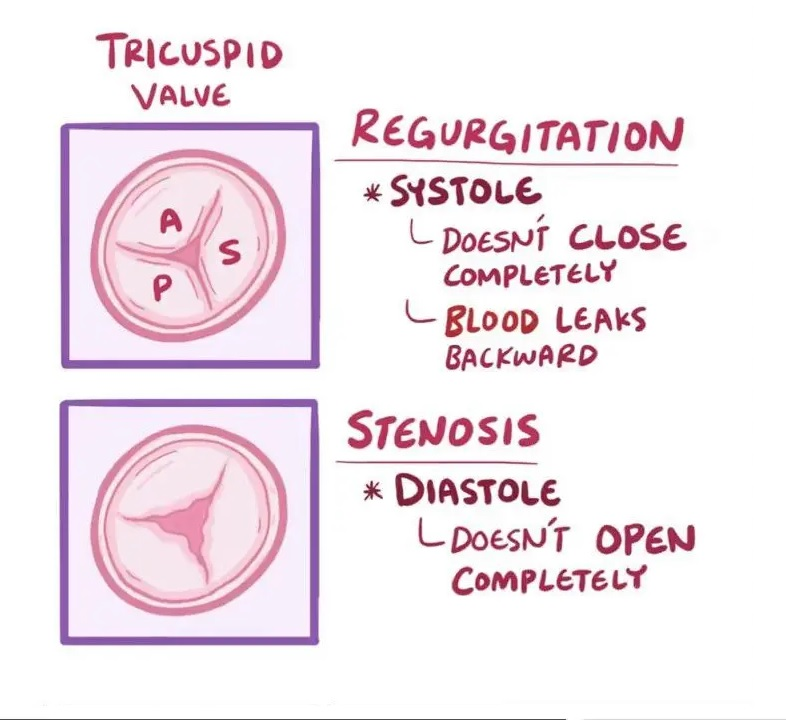
\includegraphics[width=\linewidth]{figures/regurgsteno.jpg}
    \captionof{figure}{Illustration of Regurgitation vs Stenosis ~\citeonly{TricuspidValveDisease}}
    \label{fig:regurg}
}
\begin{itemize}
    \item Valvular Stenosis: Stenosis of a valve leads to a narrowing of the valve opening, restricting blood flow. This results in increased workload for the heart chambers upstream of the affected valve, potentially causing hypertrophy and, ultimately, heart failure.
    \item Valvular Regurgitation: Valve regurgitation occurs when a valve does not close properly, allowing blood to flow backward. This leads to volume overload in the affected chambers, requiring the heart to work harder to pump the additional volume, which can also lead to heart failure over time.
\end{itemize}
Both conditions, if severe, can significantly impair cardiac function and may require surgical intervention, such as valve repair or replacement, to restore normal blood flow dynamics and prevent further cardiac damage. For instance, afterload mismatch in valvular heart disease, particularly in aortic stenosis, occurs when the left ventricle is unable to generate sufficient pressure to overcome the increased afterload caused by the stenosed valve, leading to a decrease in cardiac output. Surgical therapy, like aortic valve replacement, can relieve this mismatch and improve cardiac function, underscoring the importance of timely intervention in patients with valvular heart disease ~\citeonly{rossAfterloadMismatchAortic1985}.
\todo{maybe delete}


%     Variability and Pathologies: Briefly touch on common variations in \gls{TV} anatomy and how they might affect valve function. Also, review pathologies that can affect the valve, underscoring the need for effective simulation models.
\subsection{Variability and Pathologies}\label{sec:varpath}
The \gls{TV} is an essential component of the heart's right side and plays a critical role in the unidirectional blood flow from the right atrium to the right ventricle. Its anatomy and functioning can be affected by various factors, highlighting the importance of understanding its variability and pathologies;

\newthought{Anatomical Variability:}\\
The \gls{TV} typically features three leaflets (anterior, septal, and posterior), supported by chordae tendineae and papillary muscles. However, there can be considerable anatomical variability, including the number and size of leaflets, the structure of the subvalvular apparatus(papillary muscles, chordae tendineae and free wall), and the annular size. Such variations can impact valve function and are crucial for distinguishing between normal anatomical diversity and pathological alterations. In some instances, additional leaflets or unusual leaflet sizes are observed, affecting the valve's competence and flow dynamics. Understanding these variations is essential for accurate diagnosis and treatment planning, especially in surgical repairs and replacements .~\citeonly{tretterAssessmentAnatomicalVariation2016}

\newthought{Pathologies Affecting Valve Function:}\\
\gls{TV} pathologies can be classified into primary, involving intrinsic valve anatomy alterations, and secondary, resulting from functional modifications due to other cardiac or systemic conditions.
\begin{itemize}
    \item Primary \gls{TV} disease encompasses congenital abnormalities, infective endocarditis, rheumatic disease, and degenerative changes.
    \item Secondary \gls{TV} disease is often related to left heart diseases or pulmonary hypertension, leading to tricuspid annular dilation and right ventricular remodeling. These changes can result in tricuspid regurgitation or, less commonly, tricuspid stenosis, significantly impacting cardiac function and patient prognosis.
\end{itemize}
Advanced imaging techniques are crucial for the detailed evaluation of \gls{TV} anatomy and pathology, aiding in the accurate assessment and management of these conditions.~\citeonly{shahTricuspidValveDisease2008} One key aspect of tricuspid regurgitation that this study is looking to capture is the remodelling affects that tricuspid regurgitation has on the right ventricle and the valvular apparatus, some key variables that changes are the annular dilation, annular height, and circularity, which have been shown to increase in \citeonly{namModelingTricuspidValve2023} and chordal/papillary muscle lengths in \citeonly{obaseElongationChordaeTendineae2016}. All of these parameters are hoped to be captured over the study.

\newthought{Need for Effective Simulation Models:}\\
Given the complex anatomy of the \gls{TV} and the wide range of pathologies that can affect it, there is a growing need for effective simulation models. These models, computational and experimental can help in understanding the functional impacts of anatomical variability and pathological changes on the \gls{TV}, facilitating the development of more precise diagnostic tools and treatment strategies. Such models are particularly valuable in planning surgical interventions and predicting their outcomes.

\section{Advances in Heart Valve Disease Treatment}
%     Treatment Innovations: Review current and emerging treatments for \gls{TV} disease, including surgical interventions, transcatheter valve repair, and replacement therapies. Highlight how advancements in valve modeling and simulation could impact treatment outcomes or the development of new therapeutic techniques.
The landscape of treatments for \gls{TV} disease has been evolving, incorporating both surgical interventions and transcatheter approaches to offer alternatives for patients with varied risk profiles. Surgery remains the standard treatment for \gls{TV} disease, with techniques such as annuloplasty, leaflet repair, or valve replacement being common. However, surgical intervention is often reserved for patients without significant comorbidities due to the invasive nature of the procedures and the associated recovery times.

\newthought{Transcatheter Developments:}\\
Transcatheter techniques have emerged as a forefront innovation for treating \gls{TV} disease, especially for high-risk patients for whom traditional surgery is not viable. Transcatheter \gls{TV} repair and replacement therapies have shown promise in reducing tricuspid regurgitation and improving patient outcomes with less invasiveness than traditional surgery.
\begin{itemize}
    \item In transcatheter tricuspid valve repair various devices and techniques are being developed and tested, including coaptation devices, annuloplasty systems, and heterotopic caval valve implantation. These approaches aim to reduce tricuspid regurgitation by improving leaflet coaptation or reducing annular dilatation, offering symptomatic relief and functional improvement to patients with severe tricuspid regurgitation. ~\citeonly{hellComputedTomographyImaging2021}

    \item Transcatheter tricuspid valve replacement involves the percutaneous placement of a new valve within the native tricuspid annulus or a previously implanted surgical valve. This method has been advantageous for patients with severe \gls{TV} disease who are ineligible for surgical repair or replacement, demonstrating comparable safety and short-term outcomes. ~\citeonly{galesTranscatheterValveReplacement2018}
\end{itemize}
\begin{figure}[H]
    \centering
    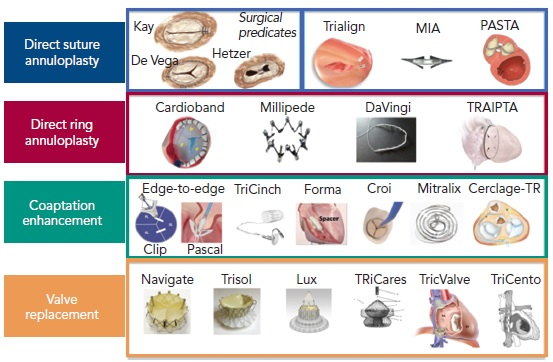
\includegraphics[width=\linewidth]{figures/TTVR.jpg}
    \caption{Current landscape of \gls{TTVR} products being used surgically ~\citeonly{curioUpdateCurrentLandscape2019}}
    \label{fig:TTVR}
\end{figure}

\newthought{Impact of Valve Modelling and Simulation:}\\
Advancements in valve modeling and simulation have significantly impacted the development of new therapeutic techniques for \gls{TV} disease. High-fidelity models created from patient-specific anatomical data have been instrumental in the design and testing of transcatheter devices, allowing for the precise customization of treatments. Computational simulations have also been crucial in understanding the biomechanical properties of the \gls{TV} under various physiological conditions, aiding in the optimization of device designs for improved durability and performance. These innovations in modelling and simulation hold the potential to enhance treatment outcomes for \gls{TV} disease, paving the way for the development of more effective and less invasive therapeutic options.

\section{Current Models and Simulators}

\subsection{Early Developments and Evolutation of Physcial Simulators}
The development of simulators in the field of cardiac care has a rich history, tracing back to the mid-20th century when the first conceptual models of blood flow dynamics and heart mechanics were introduced. These early models were primarily analog systems that used electrical circuits to mimic the hydraulic and hemodynamic properties of the heart. A pivotal innovation during this period was the development of the Windkessel model ~\citeonly{westerhofArterialWindkessel2009}, which was crucial in understanding arterial load and its effects on cardiac function, it described the haemodynamics of the arterial system in terms of resistance and compliance. It explained aortic pressure decay in diastole, but fell short in systole.
\marginpar{
    \centering
    \footnotesize
    \includegraphics[width=\linewidth]{figures/WindKessel.jpg}
    \captionof{figure}{Concept of the WindKessel Model ~\citeonly{westerhofArterialWindkessel2009}}
    \label{fig:wk}
}
The development of physical simulators has come hand in hand with clinical, computational and biological research advancements. Increases in computational power have allowed for the development of more advanced finite element models of the heart, which can simulate complex interactions between blood flow and heart valve mechanics. Software advancements have also played a critical role, with tools capable of simulating \gls{FSI} in the heart. Tangental clinical and biological studies have given more reason to develop physical simulators as now new hypotheses can be drawn from their learnings and then tested in a physical model.

The advent of 3D printing and \gls{CAD} technologies has revolutionized the fabrication of physical heart valve simulators. These technologies allow for high precision and customization of simulator components, enabling the production of complex valve geometries that accurately represent diverse anatomical variations seen in the population. This capability is vital for developing simulators that can be used for specialized surgical training and pre-surgical planning.

\subsection{Current State of the Art Simulators}

Heart valve models and simulators have significantly advanced, providing diverse tools for educational purposes, surgical planning, and research. These models range from low-fidelity simulators for basic educational use to high-fidelity, patient-specific models for complex surgical planning and research on prosthetics or interventions.

\newthought{Surgical Planning and Educational Models:}\\
Low-fidelity models, often made from commonly available materials, are used primarily for educational purposes. They provide an accessible and cost-effective means for trainees to develop surgical skills and understand valve anatomy and function. For instance, novel simulators made from components like baby bottles, combined with dental dam, offer simulation training in mitral and \gls{TV} surgical techniques, almost anywhere, at minimal cost. These models have been evaluated positively for their ability to replicate anatomy and surgical handling, proving very useful as training tools for cardiac surgery ~\citeonly{verberkmoesNovelLowfidelitySimulator2013}\\

One attempt at such an educational simulator took an entirely tissue-based approach. ~\citeonly{ramphalHighFidelityTissuebased2005} This offered a realistic environment for training cardiac surgical residents, replicating a variety of cardiac surgical procedures. They are instrumental in low-volume cardiothoracic surgery units, providing trainees with pre-clinical experience and helping them respond to clinical situations associated with heart-lung bypass machine operation and changes in patient clinical parameters.\\

Advanced, high-fidelity models are developed for surgical planning and research, employing technologies like 3D printing and silicone casting to create patient-specific valve models. These models enable simulation under dynamic physiologic conditions, allowing for the testing of surgical repairs and interventions with considerable accuracy. For example, dynamic ventricular simulators, capable of testing the quality of simulated heart valve procedures, utilize 3D printed valve suspension chambers and model pulsatile pumps to provide close-to-physiologic hemodynamic conditions for education and training in cardiac surgery ~\citeonly{zilinskasPhysiologicalVentricularSimulator2022}\\

Simulation models for valve surgery, like those for mitral valve repair, offer detailed physiological simulation, including real-time feedback mechanisms. These models incorporate integrated sensors to generate, record, and display quantitative data on trainee performance, significantly enhancing the learning experience ~\citeonly{tozziHeartSurgerySimulator2022}\\

Utilizing 3D printed valve suspension chambers and model pulsatile pumps, these simulators offer close to physiologic hemodynamic conditions. They have been validated for testing aortic valve leaflet repairs and replacements, demonstrating the potential for extensive educational use in cardiac surgery. ~\citeonly{zilinskasPhysiologicalVentricularSimulator2022}\\

Computational models are developed based on patient-specific data to predict clinical outcomes, aiding in planning medical procedures such as percutaneous pulmonary valve implantation and surgical repair of congenital heart diseases. These simulations have shown good agreement with clinical decisions, demonstrating their utility in personalized cardiovascular treatments. ~\citeonly{capelliPatientspecificSimulationsPlanning2017}

\newthought{Research-focused Models:}\\
For research, especially in developing prosthetics and testing interventions, simulators that can replicate the heart's mechanical and hemodynamic environment under various conditions are utilized. These include both native heart valve simulations and artificial heart valve simulations, categorized based on the prototype model. Such models are pivotal in studying valve biomechanics, facilitating predictive surgical planning, and aiding in the design and evaluation of repair devices and prostheses ~\citeonly{zhongNumericalSimulationDynamics2014}\\

Simulators designed to house an entire explanted heart subjected to pulsatile fluid-dynamic conditions enable the hemodynamic analysis of simulated surgical procedures. These setups are beneficial for device testing, offering a platform for in-depth investigation of valvular surgeries and interventions. ~\citeonly{leopaldiVitroHemodynamicsValve2012}


\newthought{Fidelity to Human Anatomy and Physiology in  Simulators:}\\
\begin{itemize}
    \item Some \gls{BHV}'s, such as the Texas TriValve 1.0, have made significant strides in computationally capturing the kinematics and kinetics of the native \gls{TV}. This model, reverse-engineered from a beating human heart, showcases how finite-element models can closely mimic the natural function of the \gls{TV}, including disease-induced and repair-induced changes. This level of detail offers a promising platform for simulating surgical and transcatheter interventions, aiming to improve patient outcomes. ~\citeonly{mathurTexasTriValveReverseengineered2022}
    \item Advanced simulators and models, especially those using 3D printing and computational simulations, have demonstrated a high degree of anatomical and physiological accuracy. These models can replicate complex heart valve geometries and dynamics, providing realistic conditions for training, surgical planning, and device testing. ~\citeonly{rabbahNovelLeftHeart2013}

    \item Anatomical and Mechanical Studies: Comparative studies have been crucial in understanding the mechanical, morphological, and microstructural differences between the mitral and tricuspid leaflets and chordae tendineae. These studies reveal that while there are no major differences in leaflet mechanics between the two valves, chordal mechanics can vary significantly, influenced by anatomical location and valve type. This information is vital for surgical and computational applications, especially considering the \gls{TV}'s unique stresses and strains. ~\citeonly{pokutta-paskalevaComparativeMechanicalMorphological2019}
\end{itemize}

\newthought{Paper released March 2024 - post thesis work conducted}
\begin{itemize}
    \item A research group in Heidelberg ~\citeonly{karlExvivoInvitroDynamic2024} developed a rig for mitral valve investigations in a manner similar to the aims of this project as they worked to investigate the effects of the MitraClip device. The rig was designed with less anatomical accuracy and not allowing \gls{PIV} measurement however this allowed the group to implement fixturing for motorized chordae tendineae adjustment and a camera system very close up and head-on to the valve to capture the coaptation process.
          \marginpar{
              \centering
              \footnotesize
              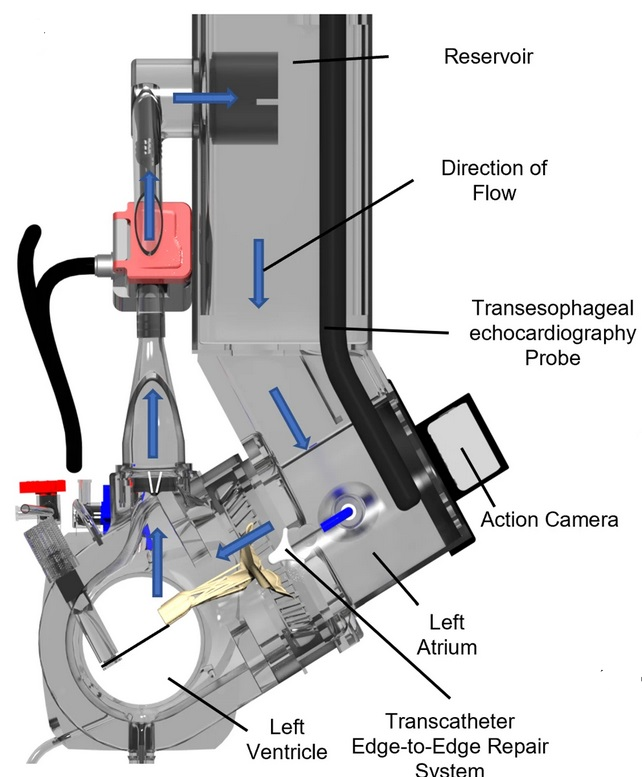
\includegraphics[width=\linewidth]{figures/karl2.jpg}
              \captionof{figure}{Side cross section of simulator with dynamic statecamera attachment ~\citeonly{karlExvivoInvitroDynamic2024}}
              \label{fig:k1}
          }
          \marginpar{
              \centering
              \footnotesize
              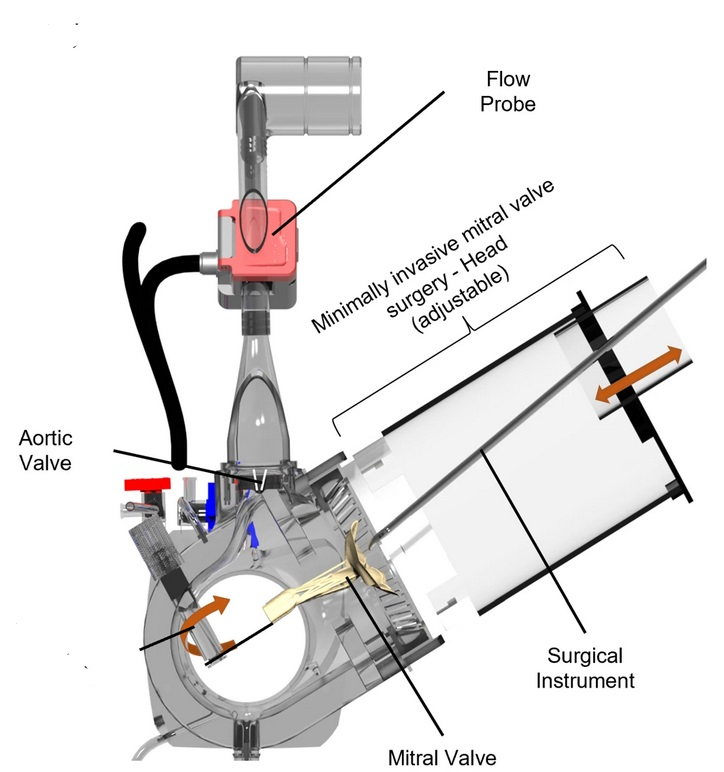
\includegraphics[width=\linewidth]{figures/karl1.jpg}
              \captionof{figure}{Side cross-section with static state surgery attachment ~\citeonly{karlExvivoInvitroDynamic2024}}
              \label{fig:k2}
          }
          This study ran a few different experiments, one with a mitral valve prosethesis, one with a mechanical valve, two with ex-vivo valves that were sewn onto an oversized elliptical frame and one experiment most close to the nature of this thesis where an in-vitro valve was
\end{itemize}
\newthought{Impact on Understanding Valve Mechanics and Patient Outcomes:}\\
Simulators play a crucial role in understanding the intricate mechanics of heart valves under various physiological and pathological conditions. They provide a risk-free environment for exploring new surgical techniques and device interventions, which is critical for advancing cardiac care. By allowing for the simulation of complex cardiac procedures and the testing of prosthetic valves and annuloplasty rings, these tools help improve surgical precision and patient outcomes. The feedback and data generated from simulators enable continuous learning and adaptation of best practices in heart valve surgery and intervention.

\section{Materials and Methods in Valve Modeling}

\subsection{Materials Used in Valve Modeling}
The development of heart valve models utilizes a range of materials, from biological tissues to synthetic polymers. These materials are selected based on their ability to simulate the natural behavior of heart valves, which is critical for ensuring the models' effectiveness in clinical training, pre-surgical planning, and device testing.
\marginpar{
    \centering
    \footnotesize
    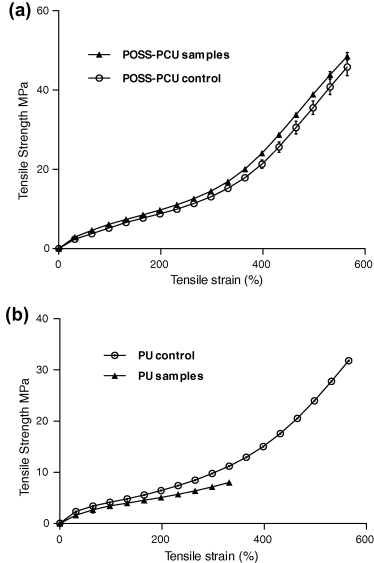
\includegraphics[width=\linewidth]{figures/PUanal.jpg}
    \captionof{figure}{Comparison of \gls{PU} and poly(carbonate-urea)urethane for heart valve performance ~\citeonly{ghanbariAnticalcificationPotentialSilsesquioxane2010}}
    \label{fig:punanal}
}
\newthought{Biological Tissues:}\\
Biological tissues have been a cornerstone in heart valve modeling, particularly for \gls{BHV} constructs. These tissues, typically derived from porcine or bovine sources, undergo treatments to enhance durability and reduce immunogenicity. The inherent biological properties of these tissues, such as their biomechanical behavior and hemocompatibility, make them suitable for simulating natural heart valve function. Limitations such as potential calcification, immune reactions have been shown however porcine and bovinepericaridium remains commonplace in current \gls{TTVR} and \gls{TAVR} respectively. ~\citeonly{filovaTissueengineeredHeartValves2009}

\newthought{Emerging Materials and Technologies:}\\
Recent advancements have led to the exploration of nanocomposite polymers \sidenote{essentially adding nano-sized building blocks into the polymer matrix which enhances durability while maintaining flexibility and processability} and hydrogels for heart valve modeling. Nanocomposite polymers, such as poly(carbonate-urea)urethane integrated with polyhedral oligomeric silsesquioxanes, exhibit enhanced mechanical properties and biostability. These materials show reduced calcification potential under in vitro conditions, making them attractive for the development of synthetic leaflet heart valves ~\citeonly{ghanbariAnticalcificationPotentialSilsesquioxane2010}

Hydrogels, derived from natural or synthetic sources, are being investigated for their potential in valve tissue engineering due to their biocompatibility and ability to support cell adhesion and proliferation. Challenges exist in balancing the bioactivity and mechanical durability of hydrogels to meet the demands of heart valve function.\citeonly{zhangApplicationHydrogelsHeart2015}

\marginpar{
    \centering
    \footnotesize
    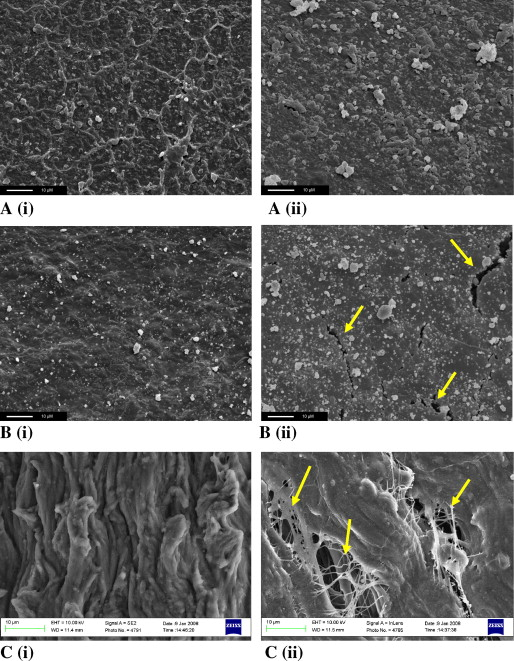
\includegraphics[width=\linewidth]{figures/PUanal2.jpg}
    \captionof{figure}{Comparison surfaces in fatigued (a) \gls{PU}  (b) poly(carbonate-urea)urethane (c) valve leaflets showing tissue failure  and fibre dehiscence marked by the yellow arrows in each ~\citeonly{ghanbariAnticalcificationPotentialSilsesquioxane2010}}
    \label{fig:puanal2}
}

\subsubsection{Synthetic Polymers:}
Synthetic polymers offer an alternative to biological tissues with advantages in consistency, durability, and the potential for customization. Polyurethane, silicone rubber, and \gls{PET} are among the polymers explored for heart valve modeling. Polyurethane, in particular, has shown promise due to its excellent tear resistance and similarity to the mechanical properties of natural valve tissue. The flexibility and durability of \gls{PU} make it an appealing choice for synthetic heart valve leaflets, though challenges remain in mimicking the viscoelastic properties of natural valves. ~\citeonly{baxterChapter12Selection2006} \sidenote{In the context of this project, choosing a synthetic material is desirable due to the intrinsic need of longevity so finding a \gls{PU} similar to those in valve replacements that can mimic the \gls{TV}'s function is}

\newthought{Silicone Mitral Valve Study}
The Engelhardt group \citeonly{engelhardtFlexibleComprehensivePatientspecific2019}
\begin{figure}[H]
    \centering
    \href{https://link.springer.com/article/10.1007/s11548-019-01971-9#MOESM1}{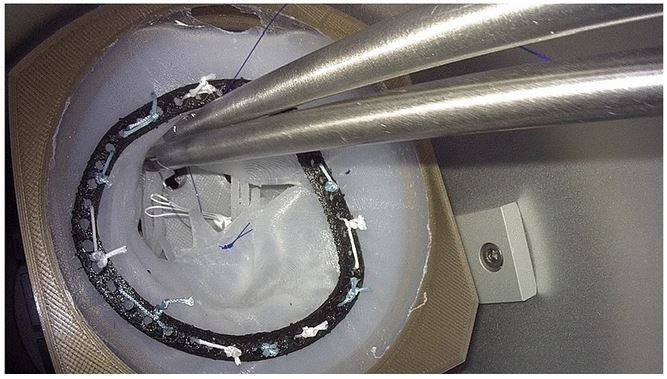
\includegraphics[width=\linewidth]{figures/Engel}}%
    \caption{Video of annuloplasty being performed on silicone mitral valve \textbf{(click to view video)}}
    \label{fig:Videoengel}
\end{figure}

\newthought{}
\citeonly{gintyModelingPatientSpecificDeformable2018}

\todo{finish this paper disc}
\newthought{Polyurethane Mitral Valve Study}
\citeonly{luoEffectBendingRigidity2012}
0.125mm average thickness, chordae 0.7mm diam, modelled in systole, leaflet youngs modulus 5.4mpa\ chordae youngs 30mpa

small Youngs modulus (~0.5 MPa) and high extensibility (~900\%) of the silicone alone. MV structures such as primary chordae tendineae have a higher Youngs modulus (~85 MPa) and a lower extensibility (4.3\%)\citeonly{liaoStructuralBasisSizerelated2003}



% \subsection{3D Printing and Fabrication Techniques}
%     3D Printing and Fabrication Techniques: Dive into modern fabrication techniques, especially 3D printing, used in valve model creation. Discuss the advantages of these methods in achieving anatomical precision and customizability.


\subsection{From Anatomical Data to Model}
%     From Anatomical Data to Model: Explain the process of translating anatomical data (e.g., from \gls{CT} scans, MRI) into functional models. Discuss the importance of accurate data and advanced imaging techniques in creating realistic models.
\newthought{Precedent of left heart valve models:}\\
In the process of translating anatomical data from \gls{CT} scans and \gls{MRI} into functional heart valve models, researchers have developed sophisticated methods to accurately capture the complex geometry and dynamics of the heart's valvular apparatus. This transition from imaging data to practical, patient-specific models is pivotal in advancing cardiac care, offering insights for surgical planning, device testing, and personalized treatment strategies.

~\citeonly{ionasecPatientSpecificModelingQuantification2010} introduced one of the first automatic computational systems for patient-specific modeling and quantification of the left heart valves, operating on cardiac \gls{CT} and transesophageal echocardiogram data. Their method, leverages discriminative learning and estimates  parameters from volumetric slices, enabling a holistic representation of the aortic and mitral valves that accounts for anatomical variations.

In a similar vein, ~\citeonly{grbicCompleteValvularHeart2012} proposed a patient-specific model of cardiac valves from 4D cardiac \gls{CT} data. Their model addresses the anatomical, functional, and hemodynamic aspects of the heart, utilizing a constrained Multi-linear Shape Model conditioned by anatomical measurements. This approach offers a more detailed representation of the heart's valvular structures and dynamics, facilitating the study of valvular pathologies and interventions.

\todo{Finish this paper disc}
One research group has done multiple studies on making anatomical models for procedure planning and device testing. The group 3d printed semi flexible material to implant the MitraClip device\citeonly{vukicevic3DPrintedModeling2017} and later did the same for the tricuspid valve \citeonly{vukicevicPatientSpecific3DimensionalPrinted2020}

\newthought{Challenges with Right Heart:}\\
The challenges of the right heart stem primarily from the complex anatomical and functional nature of the \gls{TV}, which can be more difficult to capture accurately due to several factors:

\begin{itemize}
    \item The \gls{TV}'s structure includes multiple leaflets (usually three) and a complex subvalvular apparatus, which are not symmetrically arranged. This complexity makes it harder to capture and model accurately using standard imaging techniques compared to the more symmetrically structured mitral valve.

    \item Both CT and MRI rely on good contrast resolution to differentiate between structures. The right heart's lower pressure and flow conditions can result in poorer contrast enhancement of the \gls{TV}, further complicating accurate imaging and subsequent modeling.~\citeonly{ahnTricuspidValveImaging2021}

    \item The tricuspid valve is subject to significant motion during the cardiac cycle, and capturing its dynamic behavior accurately with CT and MRI is challenging due to potential motion artifacts.~\citeonly{suhWholeheartMotioncorrectionAlgorithm2017}
\end{itemize}

\mynewline
While these challenges have slowed progress, research on the right-heart is catching up and with techniques like \gls{CT} motion-correction algorithms and wide-detector \gls{CT} with low radiation doses ~\citeonly{ahnTricuspidValveImaging2021, suhWholeheartMotioncorrectionAlgorithm2017} so the benefits of patient specific modeling can be extended to the right heart as well.


\subsection{Evaluation and Testing Methods}
%     Evaluation and Testing Methods: Conclude by discussing how valve models are evaluated and tested for their functionality. Include methodologies for assessing their mechanical properties, durability, and physiological accuracy in simulating heart valve dynamics.
The evaluation and testing of heart valve models are crucial to ensure their functionality, mechanical properties, durability, and physiological accuracy. Several methodologies have been developed to assess these aspects, employing both in vitro and computational simulation techniques.

\newthought{Mechanical Properties and Durability Testing:}
\begin{itemize}
    \item Bench Testing to ISO Standards: ~\citeonly{stasiakDesignDevelopmentTesting2020} reported on the design, development, and testing of a polymeric heart valve, including bench testing according to ISO 5840:2015 standards. Their study highlights the importance of rigorous bench testing in evaluating valve hydrodynamics, durability (tested to over 1.2 billion cycles), and preliminary biocompatibility in short-term animal models. This comprehensive approach ensures that new valve designs meet international safety and performance standards before clinical application.
          \marginpar{%
              \footnotesize
              \textbf{Resources:}\\
              \begin{itemize}
                  \item \href{https://www.iso.org/obp/ui/en/\#iso:std:iso:5840:-1:ed-2:v1:en}{Revised ISO Overview}
              \end{itemize}
          }
    \item In Vitro Testing: ~\citeonly{walkerVitroEvaluationMechanical2010} developed a novel test chamber for an automated mock circulatory loop to evaluate the mechanical performance of heart valves. This method allows for the simulation of physiological flow conditions to assess valve functionality, durability, and potential thrombotic and hemolytic effects. Such setups are vital for understanding how artificial heart valves would perform under real-life conditions.
    \item ~\citeonly{thomasComputationalMultiscaleApproach2019} implemented a multiscale modeling approach to predict extracellular matrix microstructural changes in response to tissue-level mechanical stimuli in the \gls{TV}'s anterior leaflet. This study highlighted the importance of understanding microstructural alterations under mechanical loading for developing new tissue-engineered replacements.
\end{itemize}

\newthought{Physiological Accuracy and \gls{FSI} Models:}
\begin{itemize}
    \item  ~\citeonly{leeFluidStructureInteractionModels2020} developed dynamic computer models of \gls{BHV}s in an experimental pulse duplicator, based on the immersed boundary method for \gls{FSI}. These models simulate porcine tissue and bovine pericardial BHVs under conditions used to assess performance in commercial and custom pulse duplicators. The agreement between computational simulations and experimental data for bulk flow rates, pressures, and valve opening areas underscores the potential of \gls{FSI} modeling in valve design and evaluation.
    \item  ~\citeonly{damoreHeartValveScaffold2018} introduced double component deposition, an electrodeposition technique for fabricating valve scaffolds with controlled macro-scale morphology, mechanics, and micro-structure. This method allows for the creation of fully assembled stent-less multi-leaflet valves, demonstrating the capability of emerging fabrication techniques in producing scaffolds that closely mimic natural valve behavior.
    \item ~\citeonly{laurenceInvestigationRegionalVariations2019} conducted an investigation into the regional variations in the biaxial mechanical properties and stress relaxation behaviors of porcine atrioventricular heart valve leaflets. Their findings underscored the significance of accounting for regional differences in valve biomechanics to refine computational models for predicting diseased or surgically altered valve function. This approach allows for a more accurate simulation of heart valve dynamics and mechanical behavior under varying physiological conditions.
\end{itemize}







% Materials and Methods in Valve Modeling
%     Materials Used in Valve Modeling: Review the variety of materials used in constructing heart valve models, from biological tissues to synthetic polymers. Discuss the properties that make certain materials more suitable for simulating the natural behavior of heart valves.

\section{Regulatory and Ethical Considerations}

\subsection{Regulatory Standards for Valve Models and Simulators}
%     Regulatory Standards for Valve Models and Simulators: Discuss the regulatory environment surrounding the development and use of heart valve models and simulators, especially those intended for clinical training or pre-surgical planning. This may include standards for accuracy, safety, and efficacy.
The development and use of heart valve models and simulators, particularly those intended for biomedical engineering or pre-surgical planning, are governed by a comprehensive regulatory environment. This framework ensures that these tools meet stringent standards for accuracy, safety, and efficacy before being implemented in clinical settings.

\newthought{Experimental Validation and ISO Standards:}\\
The experimental validation of cardiac simulators, as described by ~\citeonly{bazanExperimentalValidationCardiac2016}, is a critical step in developing prosthetic heart valves. Their work underscores the importance of adhering to physiological conditions and meeting the requirements of ISO 5840 standards, which set global benchmarks for cardiovascular implants and cardiac valve prostheses. This ensures that simulators provide a suitable environment for testing valve performance in the mitral, aortic and tricuspid positions under varying heart rates.

% \newthought{Animal Models for Regulatory Compliance:}\\
% Preclinical testing in appropriate animal models is mandated by regulatory bodies like the Food and Drug Administration before human clinical trials. This in vivo testing, performed under strict regulatory guidelines, is essential for assessing the performance, durability, and biocompatibility of novel heart valve therapies. The careful selection of animal models and adherence to guidelines ensure the collection of relevant data while minimizing potential distress or discomfort to the test subjects, facilitating the transition from preclinical to clinical studies. ~\citeonly{ahlbergAnimalModelsCardiac2013}
\newthought{Safety Regulations:}\\
While physical simulators are not used within patients, they must still adhere to safety regulations to ensure they pose no hazard during use. This includes mechanical, chemical and electrical safety standards, especially for those simulators that involve interactive components or electronic devices. Regulators might require that these devices be certified safe for use in educational environments, involving regular maintenance and safety checks as well as proper training for users, personal protective equipment availability and general workplace safety.

\newthought{Living Heart Project and Integrative Simulators:}\\
The Living Heart Project represents a significant advancement in simulating human heart function through a four-chamber heart model. This integrative simulator showcases the potential of computational models of the whole heart, including its valves. Such initiatives illustrate how regulatory standards can evolve to include advanced computational methods and integrative simulators for heart valve research and development ~\citeonly{baillargeonLivingHeartProject2014} and how other research work can contribute to new regulatory standards and set a precedent for how future heart valve simulators should be conducted.

% \newthought{Considerations for Engineered Tissue Heart Valves:}\\
% The development pathway for tissue-engineered heart valves  presents unique regulatory challenges. ~\citeonly{zhangPreclinicalAssessmentCardiac2019} review the regulatory framework for medical devices and highlight the special considerations for tissue-engineered heart valves, emphasizing the importance of adhering to ISO 5840 guidelines and proposing a translational roadmap to navigate the complex regulatory environment. This underscores the necessity of a well-defined regulatory approach to ensure the safety and efficacy of emerging valve technologies.


\subsection{Ethical Implications}
%     Ethical Implications: Briefly touch on the ethical considerations in developing and deploying new heart valve treatments, with an emphasis on patient safety, informed consent, and access to innovation.
% The development and deployment of new heart valve treatments involve a complex interplay of ethical considerations. These considerations encompass ensuring patient safety, obtaining informed consent, and ensuring equitable access to innovations. Below are key points highlighting these ethical dimensions:
% \newthought{Patient Safety:}\\
% The paramount concern in the development of new heart valve treatments is patient safety. ~\citeonly{rajabChapterIIIEthical2013} delve into the ethical principles applied to biomedical research and development, emphasizing the necessity of prioritizing patient welfare throughout the development process of new prosthetic heart valves. Ensuring the safety of these innovations requires rigorous clinical trials and continuous monitoring for adverse effects post-implementation.
% \newthought{Informed Consent:}\\
% Obtaining informed consent is a critical ethical obligation when deploying new heart valve treatments. ~\citeonly{fletcherCardiacTransplantsArtificial1983} discusses the ethical framework within which medical decisions, including those relevant to cardiac transplantation and artificial hearts, are made, highlighting the importance of patient autonomy and informed decision-making. This involves ensuring that patients are fully aware of the potential risks and benefits of new treatments.
% \newthought{Access to Innovation:}\\
% Ensuring equitable access to innovative heart valve treatments is a significant ethical concern. ~\citeonly{aultmanEthicsRepeatHeart2018} examine the ethical issues surrounding repeat heart valve replacement surgery, particularly for patients with substance use disorders. This discussion extends to the broader issue of access to new and potentially life-saving treatments, irrespective of a patient's socio-economic status or other personal circumstances.
The development and deployment of physical heart valve simulators involve significant ethical considerations, especially concerning patient safety, informed consent, and access to innovative technologies.

\newthought{Patient Safety:}\\
The primary concern in the development of new heart valve simulators is to ensure patient safety. As these simulators are used in educational and pre-surgical planning, it is crucial that they accurately mimic human physiology to prevent potential errors during actual surgeries. Ensuring the safety and efficacy of these simulators involves rigorous testing and validation processes to avoid any adverse consequences during training sessions or surgical planning.~\citeonly{rajabChapterIIIEthical2013}

\newthought{Informed Consent:}\\
Although physical simulators are not implanted in patients, obtaining informed consent is crucial when they are used in scenarios that involve patient interaction, such as educational demonstrations or pre-surgical planning. Patients and participants should be fully informed about the procedures being simulated, the use of their data (if applicable), and the nature of the demonstrations to uphold ethical standards of autonomy and consent.~\citeonly{fletcherCardiacTransplantsArtificial1983}

\newthought{Access to Innovation:}\\
Access to high-quality educational tools and advanced simulators should be equitable to ensure that all medical professionals, regardless of their institution's economic status, have the opportunity to train with the best available tools. This is essential for maintaining high standards of healthcare globally and ensuring that advancements in medical training are accessible to all healthcare providers, thus broadening the benefits of innovative educational simulators.~\citeonly{aultmanEthicsRepeatHeart2018}

By addressing these ethical considerations, developers and users of heart valve simulators can ensure that their use in medical education and surgical planning is both effective and ethically sound, supporting the broader goals of improving patient care and surgical outcomes.

\section{Research Strengths and Gaps}

\subsection{Research Strengths}

\newthought{Advancements in Imaging and Computational Simulations:}\\
Recent years have witnessed significant advancements in imaging techniques and computational simulations, which have enhanced the understanding and modeling of heart valve mechanics. High-resolution imaging modalities such as 4D \gls{CT} and \gls{MRI} have enabled detailed anatomical and functional assessments of heart valves in real time. These advancements have facilitated the development of more accurate computational models that can predict how valves behave under various physiological and pathological conditions. Such models are invaluable for both pre-surgical planning and the design of prosthetic valves.

\newthought{Integration of Patient-Specific Data into Valve Design:}\\
The incorporation of patient-specific anatomical data into the design and testing of heart valves is a major strength in current research which can significantly enhance the efficacy and safety of treatments as outcomes can be predicted. This approach has led to the development of customized prosthetic valves as opposed to one-size-fits-all valves where there is increased risk of failure.~\citeonly{kidaneCurrentDevelopmentsFuture2009}

% \newthought{Development of Hybrid Models and Simulation Platforms:}\\
% Another key strength is the development of hybrid simulation models that combine both physical and computational elements. These hybrid platforms enable simultaneous analysis of mechanical and fluid dynamics aspects of valve operation, providing a comprehensive understanding of valve behavior under different conditions. Such models are crucial for the testing and verification of heart valve designs before they are used in clinical settings, ensuring that they meet the required performance standards.~\citeonly{yoganathanHybridApproachHeart2017}

\newthought{Regulatory and Standardization Advances:}\\
The establishment of standardized testing protocols and regulatory guidelines for heart valve devices is another significant strength. This regulatory framework supports innovation while ensuring patient safety and the reliability of heart valve products on the market. By adhering to these standards, researchers and manufacturers can develop and test heart valve devices more effectively.


\subsection{Research Gaps}

\newthought{Anatomical Variability:}\\
The significant anatomical variability of the \gls{TV} presents challenges in creating universally applicable models. For example, the presence of additional leaflets or variations in chordae tendineae and papillary muscles can significantly impact valve function and complicate the design of surgical interventions or prosthetic valves. Understanding and incorporating this variability into models remains a challenge.~\citeonly{tretterAssessmentAnatomicalVariation2016}

Being able to, with the same piece of equipment, account for changes like these in real-time would be greatly beneficial to studies on the \gls{TV} devices and interventions.

\newthought{Material Properties and Biomechanics:}\\
Accurately simulating the material properties and biomechanical behavior of the TV leaflets and subvalvular apparatus is complex. Finite element modeling studies have attempted to address this by adjusting material parameters and considering different collagen fiber distributions. However, these models still face limitations in accurately representing shear behavior and the complex interactions within the TV apparatus under various physiological and pathological conditions.~\citeonly{stevanellaFiniteElementModelling2010}

Developing materials that can mimic the viscoelastic properties of natural valve tissues and withstand the mechanical stresses of long-term operational testing is a critical gap in the field. This would afford researchers the time to gather more data on the same specimens in testing, increasing the reliability and statistical significance of the results.

\newthought{Dynamic Bench-Top Simulation Capabilities:}\\
Enhancing the dynamic response of simulators to replicate real-time cardiac motions and valve mechanics accurately. This includes the ability to simulate different heart rates, pressures, and pathological conditions to understand their impacts on valve function and durability as well as materials that accurately mimic the biomechanical properties of natural heart tissues, which is challenging due to the complex nature of biological tissues. These materials need to withstand the mechanical stresses of long-term operation to be effective for training and testing.

Current simulators have often opted for integrating disected porcine hearts into their setups rather than developing synthetic materials which can only withstand a very limited amount of testing before failure. This is a significant gap in the field as it limits the ability to perform long-term projects investigating aspects of valve design and function.
% \newthought{Weaknesses and Areas for Improvement:}

% \begin{itemize}
%     \item Material Properties and Biomechanics: Despite advancements, accurately simulating the material properties and biomechanical behavior of heart valves remains a challenge. There's a need for models that more accurately reflect the viscoelastic properties of valve tissues, which are critical for predicting long-term device performance and valve behavior under physiological conditions.
%     \item Dynamic Simulation Capabilities: Many models still struggle with simulating the dynamic interactions between blood flow and valve motion, especially under varying physiological conditions. Enhancing \gls{FSI} simulations would improve the realism of simulations and the predictive value of models for surgical and interventional planning.
%     \item Anatomical Variability: While patient-specific modeling has advanced, there's still a need to better account for the wide range of anatomical variability observed in heart valve structures among different individuals. Models and simulators must be adaptable to reflect this diversity accurately.
%     \item Long-term Durability and Failure Modes: Current simulators and models primarily focus on short-term functionality without adequately simulating long-term wear, material degradation, or failure modes of valves and valve replacements. Developing models that can simulate years of operation within a short time frame would be invaluable for predicting valve durability and identifying potential failure mechanisms.
% \end{itemize}

% \newthought{Innovations Needed:}
% \begin{itemize}
%     \item {Advanced Materials:}\\
%           Research into new materials that mimic the complex biomechanical properties of native valve tissues could improve the realism and predictive capability of valve models.
%     \item {Hybrid Simulation Approaches:}\\
%           Combining computational models with physical simulators could offer a more comprehensive approach to understanding valve mechanics and interventions, allowing for simultaneous assessment of anatomical, physiological, and biomechanical factors.
%     \item{Machine Learning and AI Integration:}\\
%           Leveraging machine learning algorithms to analyze outcomes from simulated valve interventions could identify patterns and predict outcomes, optimizing valve designs and surgical approaches.
%     \item{Enhanced \gls{FSI} Modeling:}\\Improving the fidelity of \gls{FSI} modeling would allow for more accurate simulations of blood flow dynamics and their impact on valve function, particularly under abnormal conditions.
% \end{itemize}


\begin{table}[H]
    \begin{fullwidth}
        \centering
        \footnotesize
        \noindent\makebox[\textwidth]{%
            % Please add the following required packages to your document preamble:
% \usepackage{multirow}

% \centering
% \begin{tabular}{p{50pt}|p{75pt}|p{75pt}|p{100pt}|p{50pt}|p{60pt}}
%     \hline
%     \textbf{Authors \& Year} & \textbf{Key Findings}                                                & \textbf{Study Objective}                                            & \textbf{Methodology}                                                                                & \textbf{Relevance to Your Study} & \textbf{Key Learnings}                        \\ \hline
%     Filová et al. 2009       & Calcification of PU in vivo                                          & Overview of tissue-engineered heart valves                          & Meta-Analysis                                                                                       & Material Choice                  & Limited sample size                           \\ \hline
%     Baxter et al. 2006       & Flexibility and durability of PU                                     & Overview of synthetic materials in heart valves                     & Tearing energy and crack growth rate tests                                                          & ~                                & Performs even better at elevated temperatures \\ \hline
%     Aggarwal et al. 2013     & Converting CT to 3D                                                  & To map patient-specific aortic valves                               & Spline-fitting with mathematic models using echocardiographic images                                & Modelling/Morphology             & Maps microstructure of leaflets               \\ \hline
%     Leopaldi et al. 2012     & Comparative data for experimental and simulatory flow-loop           & To develop a flow loop with a porcine heart                         & Endoscopic imaging and hemodynamic measured with ultrasound flowmeter and piezoelectric transducers & Simulator Development            & Compares pressures and flow rates             \\ \hline
%     Zilinskas et al. 2022    & Simulator succesfully used for performing valve replacement training & To develop a surgical training simulator using porcine aortic roots & Porcine aortic valve dissected and tether to chamber                                                & ~                                & Demonstrates efficacy of bench-top simulators \\ \hline
% \end{tabular}
% \label{littable}

\renewcommand{\arraystretch}{1.2}
\begin{tabular}{p{50pt}|p{75pt}|p{75pt}|p{110pt}|p{55pt}|p{75pt}}
  \textbf{Authors \& Year} & \textbf{Key Findings}                                                & \textbf{Study Objective}                                            & \textbf{Methodology}                                                                                & \textbf{Relevance to Your Study} & \textbf{Key Learnings}                        \\ \hline
  Filová et al. 2009       & Calcification of PU in vivo                                          & Overview of tissue-engineered heart valves                          & Meta-Analysis                                                                                       & Material Choice                  & Limited sample size                           \\
  Baxter et al. 2006       & Flexibility and durability of PU                                     & Overview of synthetic materials in heart valves                     & Tearing energy and crack growth rate tests                                                          & Material Choice                  & Performs even better at elevated temperatures \\
  Aggarwal et al. 2013     & Converting CT to 3D                                                  & To map patient-specific aortic valves                               & Spline-fitting with mathematic models using echocardiographic images                                & Modelling / Morphology           & Maps microstructure of leaflets               \\
  Leopaldi et al. 2012     & Comparative data for experimental and simulatory flow-loop           & To develop a flow loop with a porcine heart                         & Endoscopic imaging and hemodynamic measured with ultrasound flowmeter and piezoelectric transducers & Simulator Development            & Compares pressures and flow rates             \\
  Zilinskas et al. 2022    & Simulator succesfully used for performing valve replacement training & To develop a surgical training simulator using porcine aortic roots & Porcine aortic valve dissected and tether to chamber                                                & Simulator Development            & Demonstrates efficacy of bench-top simulators \\
\end{tabular}

% \centering
% \arrayrulecolor{black}
% \ADLnullwidehline
% \begin{tabular}{p{50pt}|p{75pt}|p{75pt}|p{100pt}|p{50pt}|p{60pt}}
%   \toprule
%   \textbf{Authors \& Year}                                                     & \textbf{Key Findings}                                                    & \textbf{Study Objective}         & \textbf{Methodology} & \multicolumn{1}{l!{\color{black}\vrule}}{\textbf{Relevance to Your Study}} & \textbf{Key Learnings} \\
%   \midrule
%   Filová et
%   al. 2009                                                                     & Calcification of PU in vivo                                              & Overview of tissue-engineered
%   heart valves                                                                 & \multicolumn{1}{l!{\color{black}\vrule}}{Meta-Analysis}                  & \multirow{2}{*}{Material Choice} & Limited sample size                                                                                                        \\
%   \cmidrule{1-4}\cmidrule{6-6}
%   Baxter et
%   al. 2006                                                                     & Flexibility and durability of PU                                         & Overview of synthetic materials
%   in heart valves                                                              & \multicolumn{1}{l!{\color{black}\vrule}}{Tearing energy and crack growth
%   rate tests}                                                                  &                                                                          & Performs even better at elevated
%   temperatures                                                                                                                                                                                                                                                                                                            \\
%   \midrule
%   ~Aggarwal et al. 2013                                                        & Converting CT to 3D                                                      & To map patient-specific aortic
%   valves                                                                       & Spline-fitting with mathematic
%   models using echocardiographic images                                        & Modelling / Morphology                                                   & Maps microstructure of leaflets                                                                                                                               \\
%   \midrule
%   Leopaldi
%   et al. 2012                                                                  & Comparative data for
%   experimental and simulatory flow-loop                                        & To develop a flow loop with a
%   porcine heart                                                                & Endoscopic imaging and
%   hemodynamic measured with ultrasound flowmeter and piezoelectric transducers & \multirow{2}{*}{Simulator Development}                                   & Compares pressures and flow
%   rates                                                                                                                                                                                                                                                                                                                   \\
%   \cmidrule{1-4}\cmidrule{6-6}
%   Zilinskas
%   et al. 2022                                                                  & Simulator succesfully used for
%   performing valve replacement training                                        & To develop a surgical training
%   simulator using porcine aortic roots                                         & Porcine aortic valve dissected
%   and tether to chamber                                                        &                                                                          & Demonstrates efficacy of
%   bench-top simulators                                                                                                                                                                                                                                                                                                    \\
%   \bottomrule
% \end{tabular}
% \arrayrulecolor{black}}
        \caption{Comparison of key points in the literature review}
    \end{fullwidth}
\end{table}